\chapter{Исследовательская часть}

Цель исследования — разбить данные на кластеры.

\section{Оборудование}

Характеритстики ноутбука:
\begin{itemize}
	\item процессор intel-core i5-12500H \cite{lib:intel}
	% \item ОЗУ 16 Гб DDR4
	\item ОС Windows 11 \cite{lib:windows}
\end{itemize}

\section{Результаты исследования}

\subsection{Расстояния}

\begin{figure}[H]
    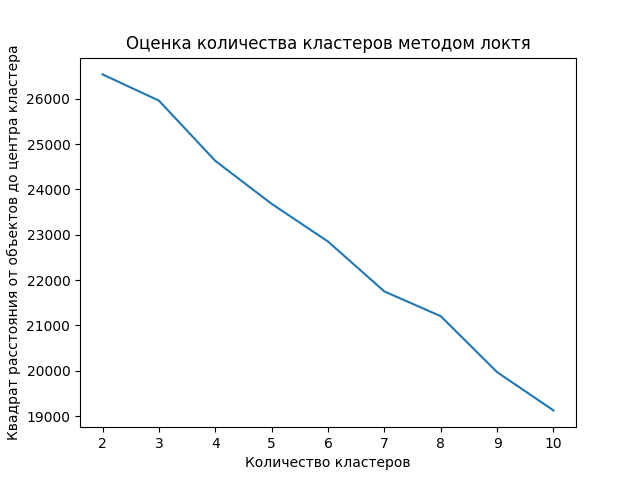
\includegraphics{C:/MGTU/baseAI/lr9/bag23u045/report/images/wcss/wcss_kmeans.png}
    \caption{Wcss oтклонения для kmeans}
\end{figure}

\begin{figure}[H]
    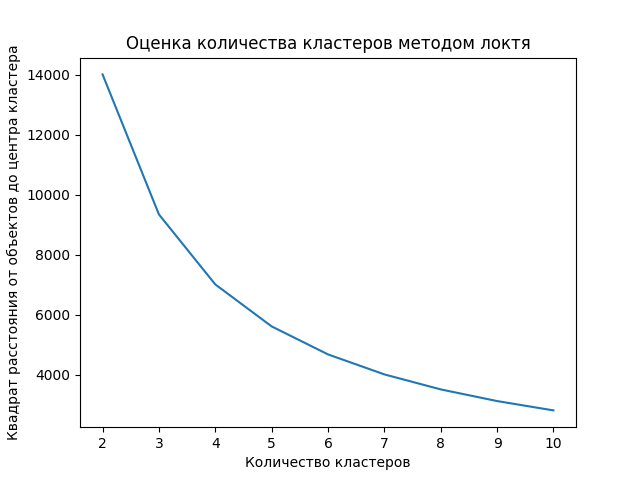
\includegraphics{C:/MGTU/baseAI/lr9/bag23u045/report/images/wcss/wcss_cmeans.png}
    \caption{Wcss oтклонения для cmeans}
\end{figure}

\begin{figure}[H]
    \centering
    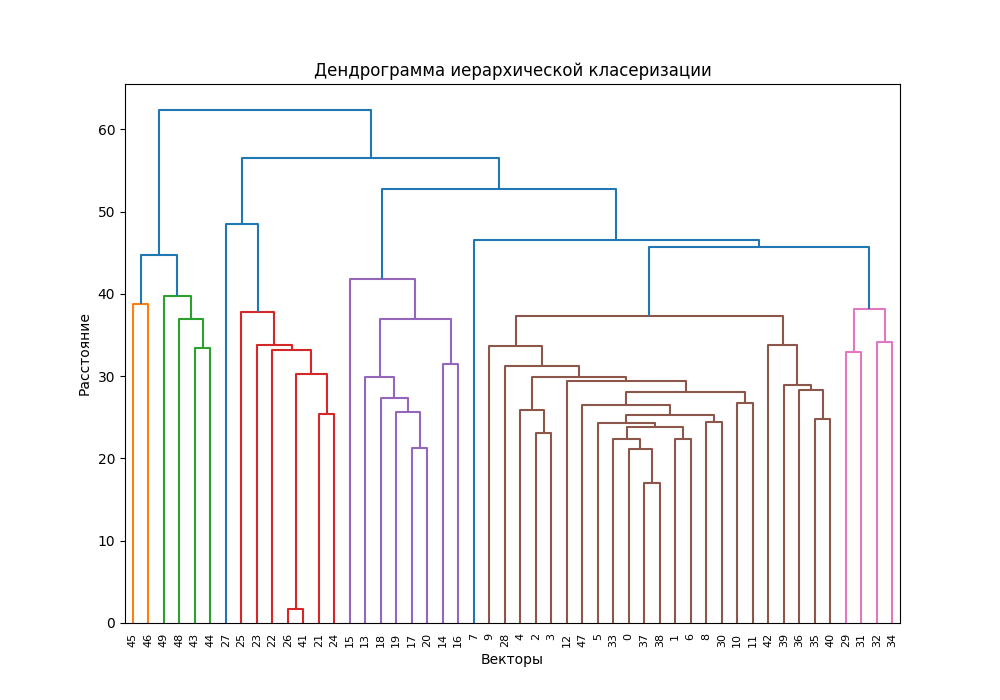
\includegraphics[width=1\textwidth]{C:/MGTU/baseAI/lr9/bag23u045/report/images/wcss/dendrogramm_ward.png}
    \caption{Дендрограмма}
\end{figure}

\begin{figure}[H]
    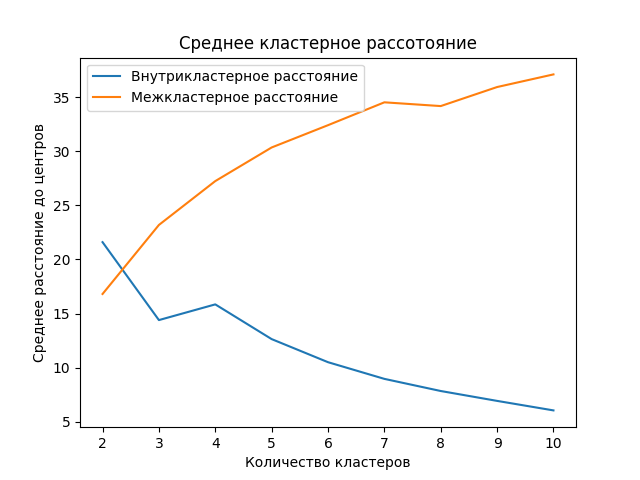
\includegraphics{C:/MGTU/baseAI/lr9/bag23u045/report/images/distance/distance_kmeans.png}
    \caption{Внутрикластерное и межкластерное расстояние для kmeans}
\end{figure}

\begin{figure}[H]
    \centering
    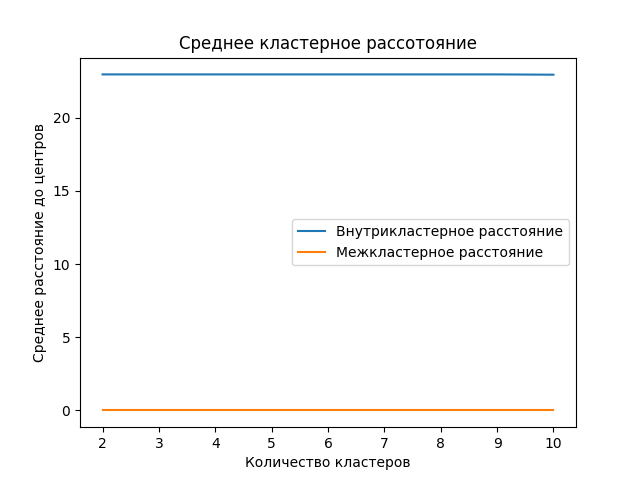
\includegraphics[width=1\textwidth]{C:/MGTU/baseAI/lr9/bag23u045/report/images/distance/distance_cmeans.png}
    \caption{Внутрикластерное и межкластерное расстояние для cmeans}
\end{figure}

\begin{figure}[H]
    \centering
    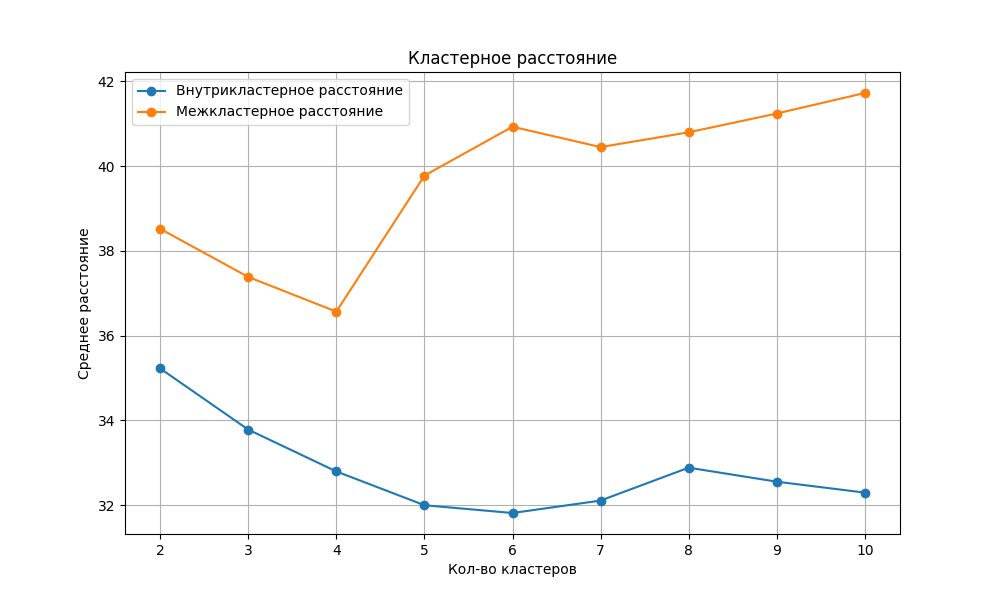
\includegraphics[width=1\textwidth]{C:/MGTU/baseAI/lr9/bag23u045/report/images/distance/cluster_distance_analysis_ward.png}
    \caption{Внутрикластерное и межкластерное расстояние для иерархической кластеризации}
\end{figure}

\subsection{Кластеры} \label{clusters}

\begin{figure}[H]
    \centering
    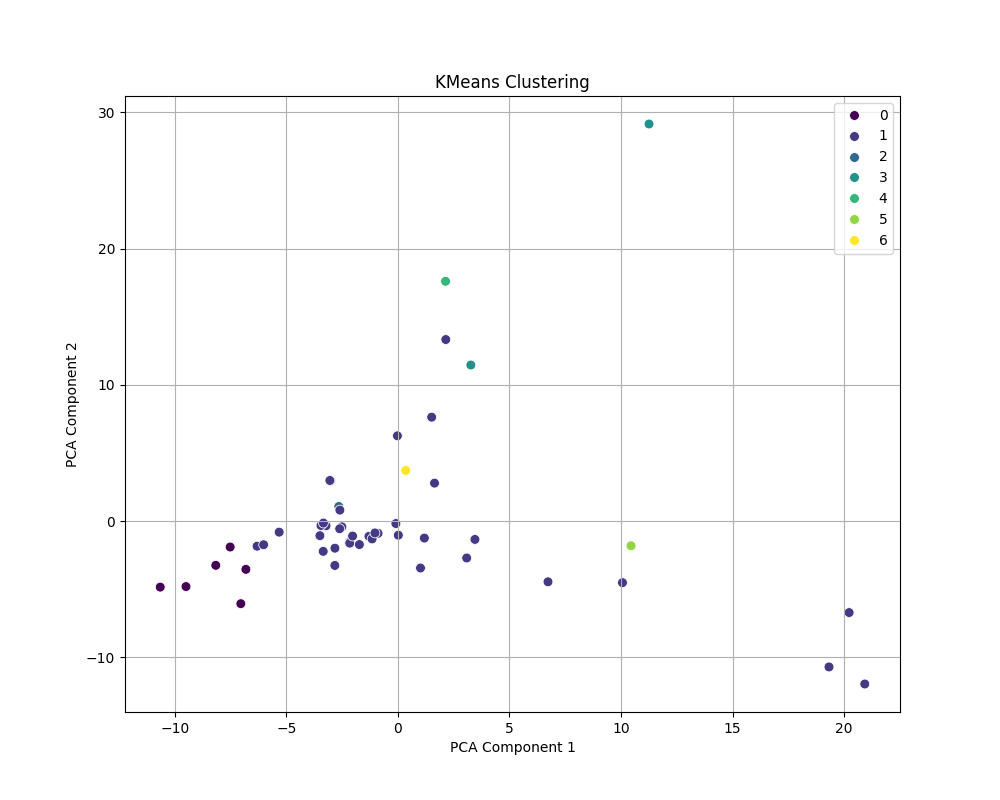
\includegraphics[width=1\textwidth]{C:/MGTU/baseAI/lr9/bag23u045/report/images/cluster/KMeans Clustering expert.png}
    \caption{Кластеры по методу kmeans (экспертная оценка)}
\end{figure}

\begin{figure}[H]
    \centering
    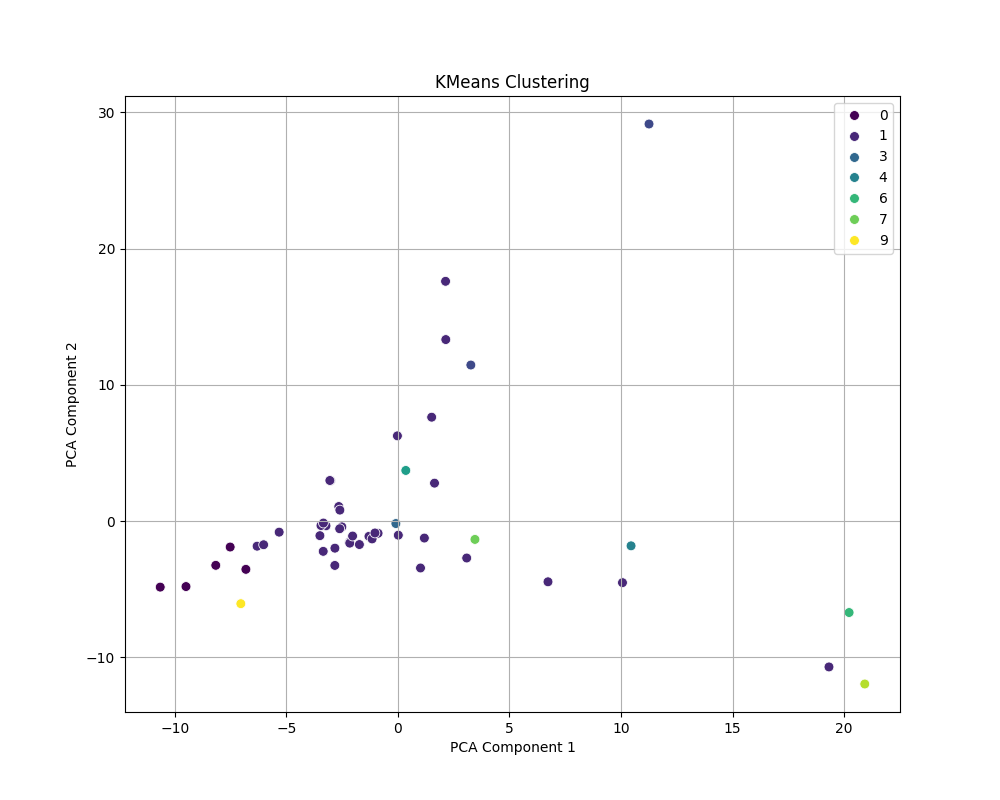
\includegraphics[width=1\textwidth]{C:/MGTU/baseAI/lr9/bag23u045/report/images/cluster/KMeans Clustering student.png}
    \caption{Кластеры по методу kmeans (оценка студента)}
\end{figure}

\begin{figure}[H]
    \centering
    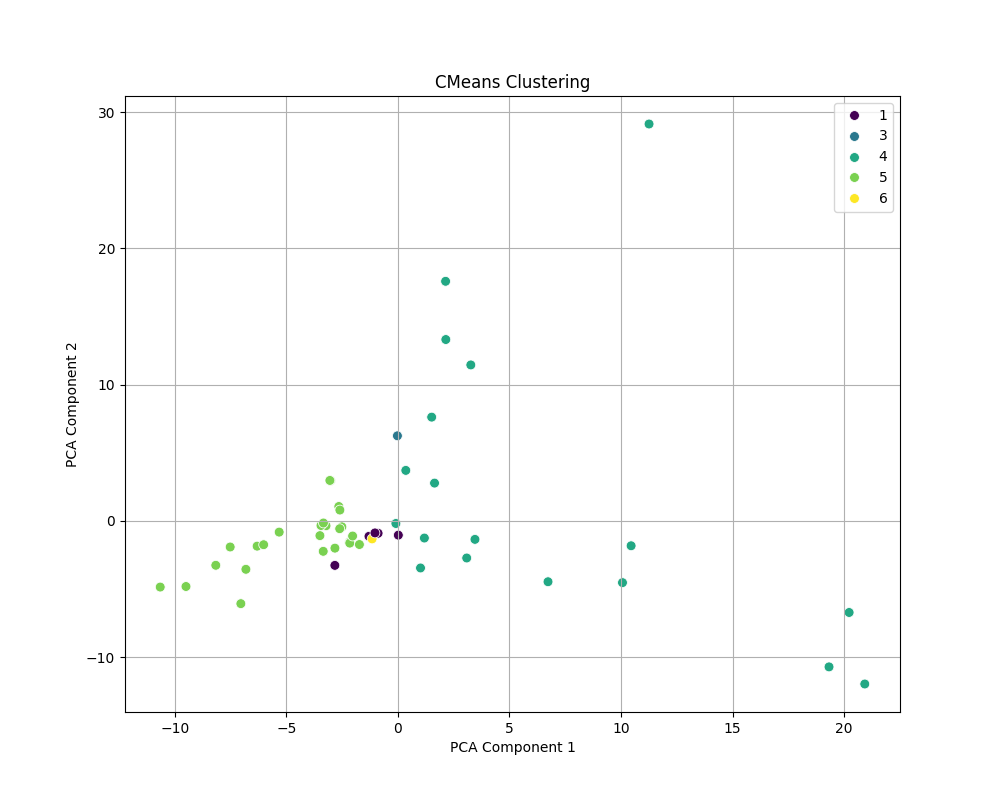
\includegraphics[width=1\textwidth]{C:/MGTU/baseAI/lr9/bag23u045/report/images/cluster/CMeans Clustering expert.png}
    \caption{Кластеры по методу cmeans (экспертная оценка)}
\end{figure}

\begin{figure}[H]
    \centering
    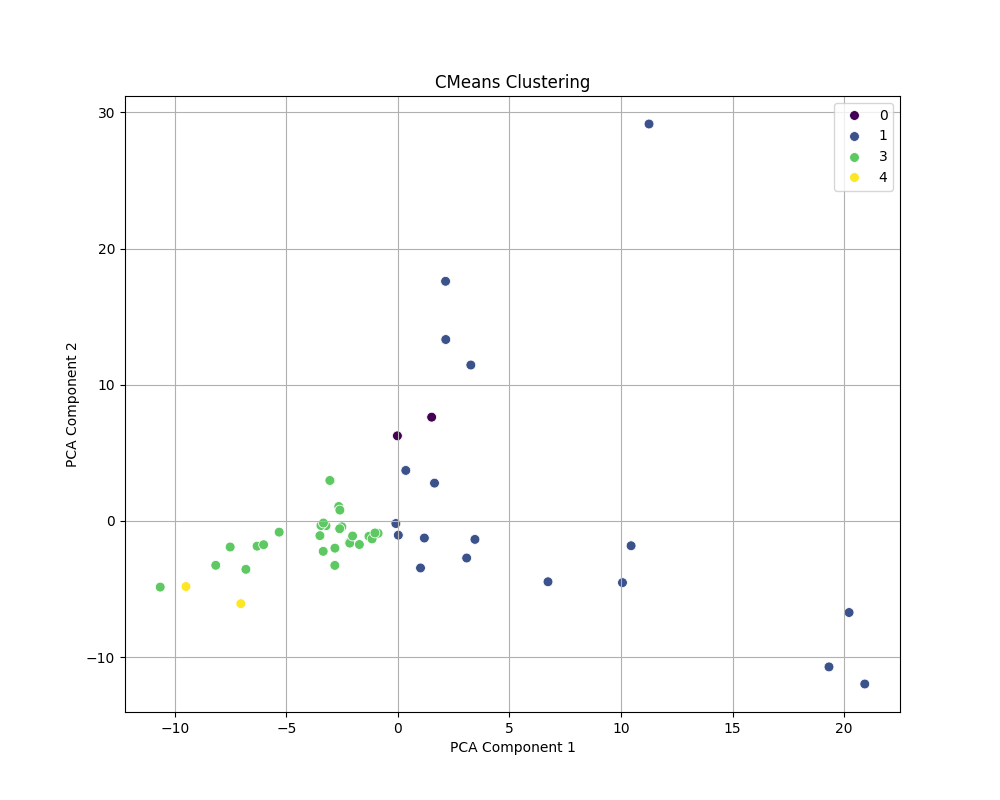
\includegraphics[width=1\textwidth]{C:/MGTU/baseAI/lr9/bag23u045/report/images/cluster/CMeans Clustering student.png}
    \caption{Кластеры по методу cmeans (оценка студента)}
\end{figure}

\begin{figure}[H]
    \centering
    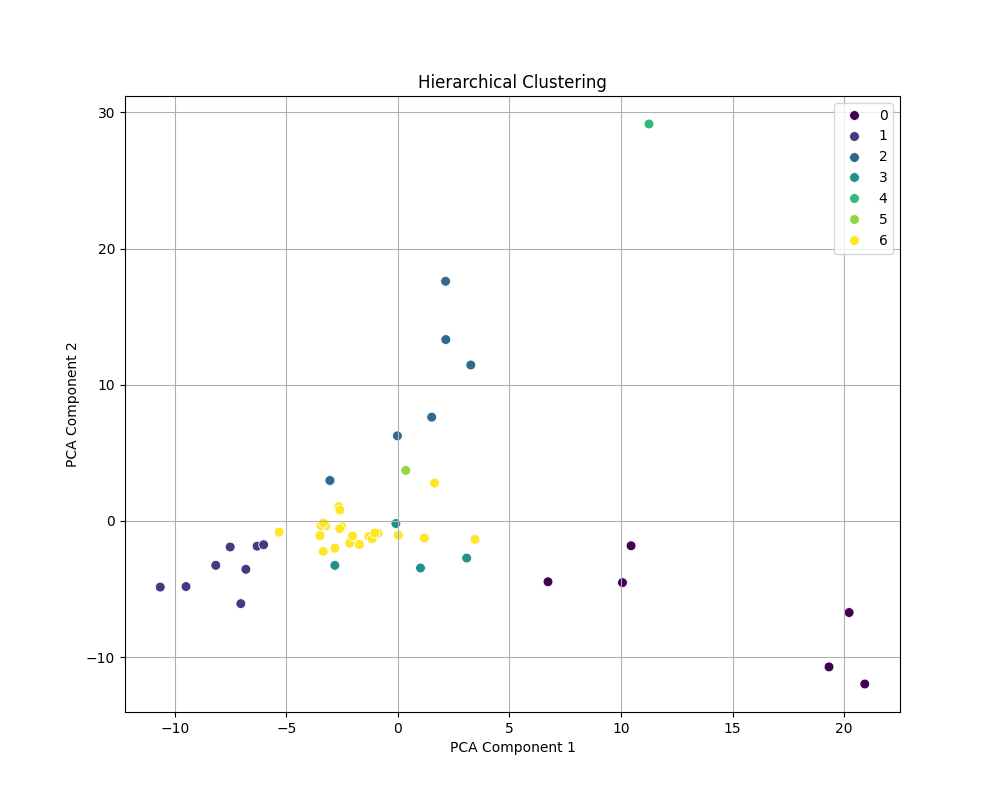
\includegraphics[width=1\textwidth]{C:/MGTU/baseAI/lr9/bag23u045/report/images/cluster/Hierarchical Clustering expert.png}
    \caption{Кластеры по методу иерархической класетризации (экспертная оценка)}
\end{figure}

\begin{figure}[H]
    \centering
    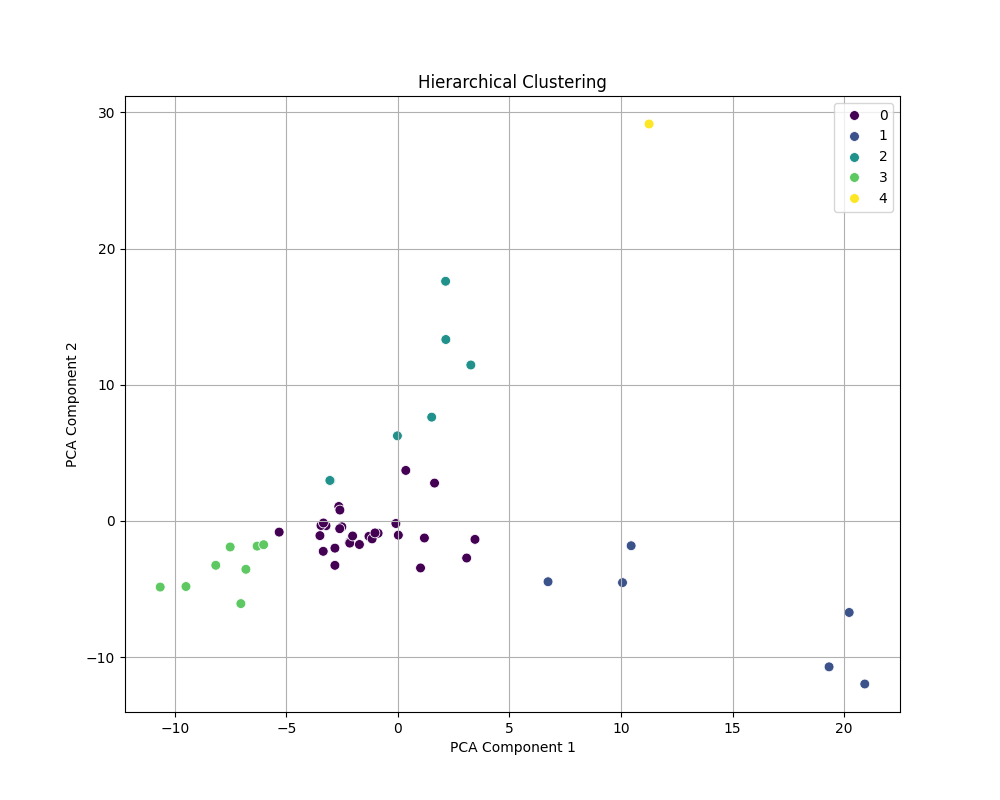
\includegraphics[width=1\textwidth]{C:/MGTU/baseAI/lr9/bag23u045/report/images/cluster/Hierarchical Clustering student.png}
    \caption{Кластеры по методу иерархической класетризации (оценка студента)}
\end{figure}

\section{Вывод}

В ходе выполнения лабораторной работы были получены графики, которые могут помочь определиться с оптимальным количеством кластеров,
а также графики, которые отражают внутрикластерное и межкластерное расстояние.
В разделе \ref{clusters} представлены результаты кластеризации методами kmeans, cmeans и иерархической кластеризации 
с количеством кластеров, определённых экспертом и студентом.

\clearpage